
%(BEGIN_QUESTION)
% Copyright 2007, Tony R. Kuphaldt, released under the Creative Commons Attribution License (v 1.0)
% This means you may do almost anything with this work of mine, so long as you give me proper credit

Offshore oil rigs and oil refineries often use {\it flare} burners to safely discharge excess product to atmosphere.  Although it seems wasteful to constantly burn off petroleum compounds in a giant outdoor burner (and it is!), it is worse to not have a safe place to vent flammable compounds in the event of an emergency shutdown requiring de-pressurization of pipes and vessels.

Flares must handle a wide variety of gases for emergency combustion.  Some of these gases burn clean, while others tend to burn ``sooty'' due to their high carbon content.  It is impossible to design a single burner assembly to efficiently and cleanly burn all manner of combustible gases, so other means are necessary to control smoke.  One such method is steam injection into the flame.  Steam increases turbulence in the flame, which promotes better air/fuel mixing for decreased smoke:

$$\includegraphics[width=15.5cm]{i01831x01.eps}$$

However, steam is an expensive commodity.  Leaving the steam valve wide-open all the time may ensure a smokeless flare, but it wastes steam when the flare is burning cleaner gases.  An automatic control system should be used to control steam flow for optimum efficiency.

One way to indirectly measure the need for steam injection in a flare is to measure radiant heat with several thermocouples (TE) arrayed near the flare tip.  Greater carbon content in a flame results in greater radiated heat, which will be sensed by the surrounding thermocouples:

$$\includegraphics[width=15.5cm]{i01831x02.eps}$$

The setpoint and/or bias of this controller is set such that the steam valve is fully closed when the radiant thermocouples' temperature is equal to ambient.  Configured as such, it is important that this controller have no integral action, only proportional and derivative.  Explain why.

\underbar{file i01831}
%(END_QUESTION)





%(BEGIN_ANSWER)

The controller should be configured for direct action, since we wish to have more steam flow for greater differential temperature.

\vskip 10pt

Note: derivative control action helps overcome lag in the thermocouple sensing elements and in the steam response by acting as a {\it lead} element.

\vskip 30pt

Since no amount of steam injection can reduce the radiant thermocouples' sensed temperature down to ambient, a controller with integral would experience reset {\it windup} under most conditions.

%(END_ANSWER)





%(BEGIN_NOTES)

Note: this control strategy derived from diagram on page 66 of Francis G. Shinskey's {\it Energy Conservation Through Control}, copyright 1978.

%INDEX% Control, strategies: differential temperature for flare smoke control
%INDEX% Process: flare anti-smoke control

%(END_NOTES)


